\documentclass{standalone}
\usepackage{tikz}
\usetikzlibrary{patterns, positioning}
\usepackage[sfdefault]{ClearSans} %% option 'sfdefault' activates Clear Sans as the default text font
\usepackage[T1]{fontenc}

\begin{document}
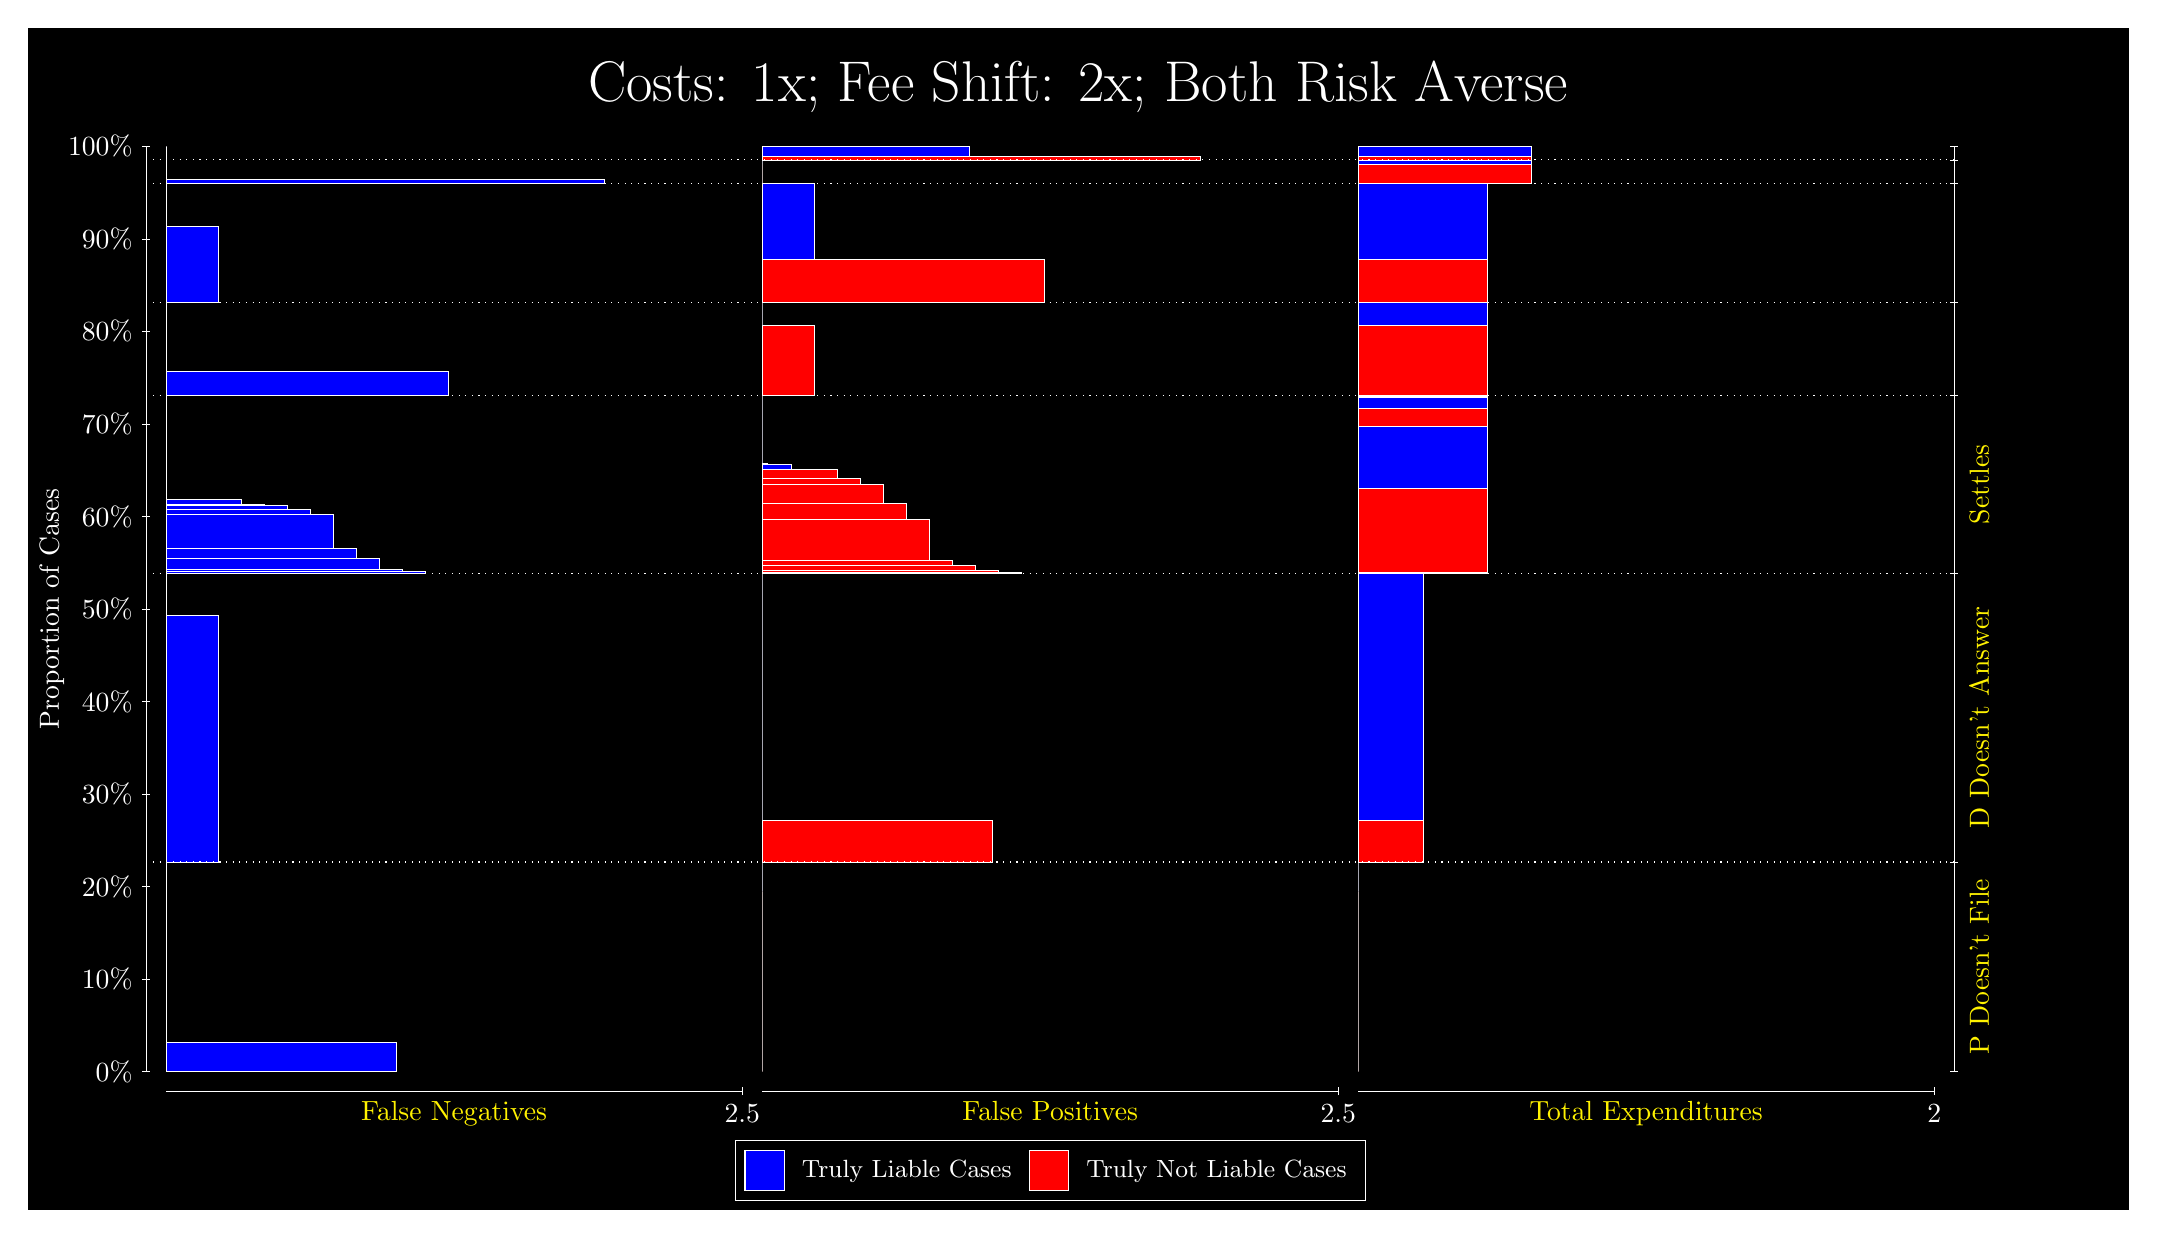
\begin{tikzpicture}
\draw[fill=black] (0,0) rectangle (26.667,15);
\draw[text=white] (0,13.5) rectangle (26.667,15) node[midway] {\huge Costs: 1x; Fee Shift: 2x; Both Risk Averse};
\draw[white, very thin] (1.5,1.75) -- (1.5,13.5);
\node[rotate=90, text=white, anchor=center] at (0.3, 7.625) {Proportion of Cases};
\draw[white, very thin] (1.45,1.75) -- (1.55,1.75);
\node[text=white, anchor=east] at (1.45, 1.75) {0\%};
\draw[white, very thin] (1.45,2.925) -- (1.55,2.925);
\node[text=white, anchor=east] at (1.45, 2.925) {10\%};
\draw[white, very thin] (1.45,4.1) -- (1.55,4.1);
\node[text=white, anchor=east] at (1.45, 4.1) {20\%};
\draw[white, very thin] (1.45,5.275) -- (1.55,5.275);
\node[text=white, anchor=east] at (1.45, 5.275) {30\%};
\draw[white, very thin] (1.45,6.45) -- (1.55,6.45);
\node[text=white, anchor=east] at (1.45, 6.45) {40\%};
\draw[white, very thin] (1.45,7.625) -- (1.55,7.625);
\node[text=white, anchor=east] at (1.45, 7.625) {50\%};
\draw[white, very thin] (1.45,8.8) -- (1.55,8.8);
\node[text=white, anchor=east] at (1.45, 8.8) {60\%};
\draw[white, very thin] (1.45,9.975) -- (1.55,9.975);
\node[text=white, anchor=east] at (1.45, 9.975) {70\%};
\draw[white, very thin] (1.45,11.15) -- (1.55,11.15);
\node[text=white, anchor=east] at (1.45, 11.15) {80\%};
\draw[white, very thin] (1.45,12.325) -- (1.55,12.325);
\node[text=white, anchor=east] at (1.45, 12.325) {90\%};
\draw[white, very thin] (1.45,13.5) -- (1.55,13.5);
\node[text=white, anchor=east] at (1.45, 13.5) {100\%};

\draw[white, very thin] (24.457,1.75) -- (24.457,13.5);
\draw[white, very thin] (24.407,1.75) -- (24.507,1.75);
\node[anchor=west] at (24.407, 1.75) {};
\draw[white, very thin] (24.407,4.4114) -- (24.507,4.4114);
\node[anchor=west] at (24.407, 4.4114) {};
\draw[white, very thin] (24.407,8.0757) -- (24.507,8.0757);
\node[anchor=west] at (24.407, 8.0757) {};
\draw[white, very thin] (24.407,10.341) -- (24.507,10.341);
\node[anchor=west] at (24.407, 10.341) {};
\draw[white, very thin] (24.407,11.521) -- (24.507,11.521);
\node[anchor=west] at (24.407, 11.521) {};
\draw[white, very thin] (24.407,13.029) -- (24.507,13.029);
\node[anchor=west] at (24.407, 13.029) {};
\draw[white, very thin] (24.407,13.327) -- (24.507,13.327);
\node[anchor=west] at (24.407, 13.327) {};
\draw[white, very thin] (24.407,13.5) -- (24.507,13.5);
\node[anchor=west] at (24.407, 13.5) {};

\draw[white, very thin, fill=blue] (1.75,1.75) rectangle (4.6775,2.1229);
\draw[white, very thin, fill=red] (1.75,2.1229) rectangle (1.75,4.4114);
\draw[white, very thin, fill=blue] (1.75,4.4114) rectangle (2.4087,7.5459);
\draw[white, very thin, fill=red] (1.75,7.5459) rectangle (1.75,8.0757);
\draw[white, very thin, fill=blue] (1.75,8.0757) rectangle (5.0435,8.0988);
\draw[white, very thin, fill=blue] (1.75,8.0988) rectangle (4.7507,8.1314);
\draw[white, very thin, fill=blue] (1.75,8.1314) rectangle (4.458,8.2631);
\draw[white, very thin, fill=blue] (1.75,8.2631) rectangle (4.1652,8.4);
\draw[white, very thin, fill=blue] (1.75,8.4) rectangle (3.8725,8.8327);
\draw[white, very thin, fill=blue] (1.75,8.8327) rectangle (3.5797,8.8842);
\draw[white, very thin, fill=blue] (1.75,8.8842) rectangle (3.287,8.9409);
\draw[white, very thin, fill=blue] (1.75,8.9409) rectangle (2.9942,8.9584);
\draw[white, very thin, fill=blue] (1.75,8.9584) rectangle (2.7015,9.0141);
\draw[white, very thin, fill=red] (1.75,9.0141) rectangle (1.75,10.341);
\draw[white, very thin, fill=blue] (1.75,10.341) rectangle (5.3362,10.638);
\draw[white, very thin, fill=red] (1.75,10.638) rectangle (1.75,11.521);
\draw[white, very thin, fill=blue] (1.75,11.521) rectangle (2.4087,12.48);
\draw[white, very thin, fill=red] (1.75,12.48) rectangle (1.75,13.029);
\draw[white, very thin, fill=blue] (1.75,13.029) rectangle (7.3123,13.08);
\draw[white, very thin, fill=red] (1.75,13.08) rectangle (1.75,13.327);
\draw[white, very thin, fill=red] (1.75,13.327) rectangle (1.75,13.378);
\draw[white, very thin, fill=blue] (1.75,13.378) rectangle (1.75,13.5);
\draw[white, very thin, fill=red] (9.3189,1.75) rectangle (9.3189,4.0385);
\draw[white, very thin, fill=blue] (9.3189,4.0385) rectangle (9.3189,4.4114);
\draw[white, very thin, fill=red] (9.3189,4.4114) rectangle (12.246,4.9412);
\draw[white, very thin, fill=blue] (9.3189,4.9412) rectangle (9.3189,8.0757);
\draw[white, very thin, fill=red] (9.3189,8.0757) rectangle (12.612,8.0964);
\draw[white, very thin, fill=red] (9.3189,8.0964) rectangle (12.32,8.1102);
\draw[white, very thin, fill=red] (9.3189,8.1102) rectangle (12.027,8.1753);
\draw[white, very thin, fill=red] (9.3189,8.1753) rectangle (11.734,8.2476);
\draw[white, very thin, fill=red] (9.3189,8.2476) rectangle (11.441,8.7676);
\draw[white, very thin, fill=red] (9.3189,8.7676) rectangle (11.149,8.9728);
\draw[white, very thin, fill=red] (9.3189,8.9728) rectangle (10.856,9.2082);
\draw[white, very thin, fill=red] (9.3189,9.2082) rectangle (10.563,9.2809);
\draw[white, very thin, fill=red] (9.3189,9.2809) rectangle (10.27,9.4028);
\draw[white, very thin, fill=blue] (9.3189,9.4028) rectangle (9.6848,9.4585);
\draw[white, very thin, fill=blue] (9.3189,9.4585) rectangle (9.3921,9.476);
\draw[white, very thin, fill=blue] (9.3189,9.476) rectangle (9.3189,10.341);
\draw[white, very thin, fill=red] (9.3189,10.341) rectangle (9.9776,11.224);
\draw[white, very thin, fill=blue] (9.3189,11.224) rectangle (9.3189,11.521);
\draw[white, very thin, fill=red] (9.3189,11.521) rectangle (12.905,12.07);
\draw[white, very thin, fill=blue] (9.3189,12.07) rectangle (9.9776,13.029);
\draw[white, very thin, fill=red] (9.3189,13.029) rectangle (9.3189,13.276);
\draw[white, very thin, fill=blue] (9.3189,13.276) rectangle (9.3189,13.327);
\draw[white, very thin, fill=red] (9.3189,13.327) rectangle (14.881,13.378);
\draw[white, very thin, fill=blue] (9.3189,13.378) rectangle (11.954,13.5);
\draw[white, very thin, fill=red] (16.888,1.75) rectangle (16.888,4.0385);
\draw[white, very thin, fill=blue] (16.888,4.0385) rectangle (16.888,4.4114);
\draw[white, very thin, fill=red] (16.888,4.4114) rectangle (17.711,4.9412);
\draw[white, very thin, fill=blue] (16.888,4.9412) rectangle (17.711,8.0757);
\draw[white, very thin, fill=red] (16.888,8.0757) rectangle (18.534,8.0879);
\draw[white, very thin, fill=blue] (16.888,8.0879) rectangle (18.534,8.0952);
\draw[white, very thin, fill=red] (16.888,8.0952) rectangle (18.534,9.1608);
\draw[white, very thin, fill=blue] (16.888,9.1608) rectangle (18.534,9.9427);
\draw[white, very thin, fill=red] (16.888,9.9427) rectangle (18.534,10.178);
\draw[white, very thin, fill=blue] (16.888,10.178) rectangle (18.534,10.31);
\draw[white, very thin, fill=red] (16.888,10.31) rectangle (18.534,10.324);
\draw[white, very thin, fill=blue] (16.888,10.324) rectangle (18.534,10.341);
\draw[white, very thin, fill=red] (16.888,10.341) rectangle (18.534,11.224);
\draw[white, very thin, fill=blue] (16.888,11.224) rectangle (18.534,11.521);
\draw[white, very thin, fill=red] (16.888,11.521) rectangle (18.534,12.07);
\draw[white, very thin, fill=blue] (16.888,12.07) rectangle (18.534,13.029);
\draw[white, very thin, fill=red] (16.888,13.029) rectangle (19.083,13.276);
\draw[white, very thin, fill=blue] (16.888,13.276) rectangle (19.083,13.327);
\draw[white, very thin, fill=red] (16.888,13.327) rectangle (19.083,13.378);
\draw[white, very thin, fill=blue] (16.888,13.378) rectangle (19.083,13.5);
\draw[white, dotted] (1.5,4.4114) -- (24.457,4.4114);
\draw[white, dotted] (1.5,8.0757) -- (24.457,8.0757);
\draw[white, dotted] (1.5,10.341) -- (24.457,10.341);
\draw[white, dotted] (1.5,11.521) -- (24.457,11.521);
\draw[white, dotted] (1.5,13.029) -- (24.457,13.029);
\draw[white, dotted] (1.5,13.327) -- (24.457,13.327);
\draw[white, very thin] (1.75,1.5) -- (9.0689,1.5);
\node[text=yellow, anchor=north] at (5.4094, 1.5) {False Negatives};
\draw[white, very thin] (9.0689,1.45) -- (9.0689,1.55);
\node[text=white, anchor=north] at (9.0689, 1.45) {2.5};

\draw[white, very thin] (9.3189,1.5) -- (16.638,1.5);
\node[text=yellow, anchor=north] at (12.978, 1.5) {False Positives};
\draw[white, very thin] (16.638,1.45) -- (16.638,1.55);
\node[text=white, anchor=north] at (16.638, 1.45) {2.5};

\draw[white, very thin] (16.888,1.5) -- (24.207,1.5);
\node[text=yellow, anchor=north] at (20.547, 1.5) {Total Expenditures};
\draw[white, very thin] (24.207,1.45) -- (24.207,1.55);
\node[text=white, anchor=north] at (24.207, 1.45) {2};

\node[text=yellow, centered, rotate=90] at (24.777, 3.0807) {P Doesn't File};
\node[text=yellow, centered, rotate=90] at (24.777, 6.2435) {D Doesn't Answer};
\node[text=yellow, centered, rotate=90] at (24.777, 9.2084) {Settles};





\draw (12.978300999999998,1.5) node[draw=none] (baseCoordinate) {};
\begin{scope}[align=center]
        \matrix[scale=0.5, draw=white, below=0.5cm of baseCoordinate, nodes={draw}, column sep=0.1cm]{
            \node[rectangle, draw, minimum width=0.5cm, minimum height=0.5cm, fill=blue] {}; &
            \node[draw=none, font=\small, text=white] (B) {Truly Liable Cases}; &
            \node[rectangle, draw, minimum width=0.5cm, minimum height=0.5cm, fill=red] {}; &
            \node[draw=none, font=\small, text=white] (B) {Truly Not Liable Cases}; \\
            };
\end{scope}

\end{tikzpicture}
\end{document}